% !TeX root = ../../main.tex
% “三合一”工具样机性能测试（据《工具单独测试.docx》整理）
% 图、表编号由 main.tex 统一设置为“章-序号”（图3-x、表3-x），此处不手工编号

\subsection{样机性能测试}
\label{subsec:3in1_performance_test}

为检验“三合一”脉冲式冲刮刷集成式井筒清洁工具（以下简称“三合一”工具）各功能模块的实际工作性能，在厂内试验台与东营试验基地分别对毛刷刮管器、脉冲器、液压刮管器及旋转喷头开展了单独测试。其中，毛刷刮管器重点考核装配完成后工具的通过性以及毛刷与管壁的接触状态；脉冲器重点考核起振排量、起振压力与振动频率；液压刮管器重点考核投球激活、刮刀张开行程及刮刀回收性能；旋转喷头重点考核不同排量下喷头的旋转起动特性。试验样机的主要参数见表\ref{tab:3in1_test_params}～表\ref{tab:3in1_brush_params}。

\subsubsection{试验样机基本参数}

液压刮管器与脉冲器的基本参数见表\ref{tab:3in1_test_params}，旋转喷头的基本参数见表\ref{tab:3in1_nozzle_params}，MSQ105型毛刷刮管器的技术参数见表\ref{tab:3in1_brush_params}。

\begin{table}[t]
    \centering
    \caption{液压刮管器与脉冲器基本参数}
    \label{tab:3in1_test_params}
    {\small % 列数较多，适当缩小字号，避免超出正文版心
    \setlength{\tabcolsep}{3pt} % 减小列间距
    \renewcommand{\arraystretch}{1.4} % 增加行高，使表格不拥挤
    \begin{tabular*}{\textwidth}{@{\extracolsep{\fill}}cccccccc@{}}
        \toprule % 顶线
        代号 & 名称 & \begin{tabular}[c]{@{}c@{}}适用套管\\ 规格\end{tabular} & 
        \begin{tabular}[c]{@{}c@{}}组装外径\\ (mm)\end{tabular} & 
        \begin{tabular}[c]{@{}c@{}}最小通径\\ (mm)\end{tabular} & 
        \begin{tabular}[c]{@{}c@{}}打开压力\\ (MPa)$^{\ast}$\end{tabular} & 
        \begin{tabular}[c]{@{}c@{}}张开直径\\ (max, mm)\end{tabular} & 
        \begin{tabular}[c]{@{}c@{}}连接螺纹\\ (API)\end{tabular} \\
        \midrule % 栏目线
        YYGG-105 & 液压刮管器 & 5-1/2\inch & $\phi$114 & $\phi$25 & 65 & $\phi$130 & \begin{tabular}[c]{@{}c@{}}NC31\\ (Pin$\times$Box)\end{tabular} \\
        MCQ-105 & 脉冲器 & 5-1/2\inch & $\phi$105 & $\phi$10 & 65 & --- & \begin{tabular}[c]{@{}c@{}}NC31\\ (Pin$\times$Box)\end{tabular} \\
        \bottomrule % 底线
    \end{tabular*}}
    \par\vspace{0.3em}
    {\raggedright\small 注：$^{\ast}$打开压力为绝对压力（即地面泵压加静液柱压力），压力可调，允差为$\pm$5\,MPa；表中“---”表示该项不适用或未给出。\par}
\end{table}

\begin{table}[t]
    \centering
    \caption{旋转喷头基本参数}
    \label{tab:3in1_nozzle_params}
    \small % 9 列较宽，用小一号字避免超出页边距
    \setlength{\tabcolsep}{2pt}
    \renewcommand{\arraystretch}{1.4}
    \begin{tabular*}{\textwidth}{@{\extracolsep{\fill}}ccccccccc@{}}
        \toprule % 顶线
        \begin{tabular}[c]{@{}c@{}}外径\\ (mm)\end{tabular} & 
        \begin{tabular}[c]{@{}c@{}}总长\\ (mm)\end{tabular} & 
        \begin{tabular}[c]{@{}c@{}}喷嘴尺寸\\ (mm$\times$n)\end{tabular} & 
        \begin{tabular}[c]{@{}c@{}}工作排量\\ (L/min)\end{tabular} & 
        \begin{tabular}[c]{@{}c@{}}转速\\ (r/min)\end{tabular} & 
        \begin{tabular}[c]{@{}c@{}}工作压强\\ (MPa)\end{tabular} & 
        扣型 & 
        \begin{tabular}[c]{@{}c@{}}最大抗拉\\ (kN)\end{tabular} & 
        \begin{tabular}[c]{@{}c@{}}最大抗扭\\ ($\mathrm{kN\cdot m}$)\end{tabular} \\
        \midrule % 栏目线
        105 & 1045 & $3.175\times7$ & $100\sim500$ & $10\sim300$ & $\le70$ & NC31 & 400 & 8 \\
        \bottomrule % 底线
    \end{tabular*}
\end{table}

\begin{table}[t]
    \centering
    \caption{MSQ105型毛刷刮管器技术参数}
    \label{tab:3in1_brush_params}
    \renewcommand{\arraystretch}{1.4}
    \begin{tabularx}{0.68\textwidth}{lC}
        \toprule % 顶线
        项目 & MSQ105 \\
        \midrule % 栏目线
        本体最大外径（mm） & $\phi$110 \\
        毛刷最大外径（mm） & $\phi$130 \\
        适用套管（in） & 5-1/2\inch \\
        使用套管磅级（ppf） & $23\sim29$\# \\
        许用工作拉力，kN（lb） & 50（11200） \\
        许用工作扭矩，$\mathrm{kN\cdot m}$（lb$\cdot$ft） & 10（7200） \\
        水眼（mm） & $\phi$30 \\
        总长（mm） & 1300 \\
        接头外径（mm） & $\phi$105 \\
        接头扣（API）B$\times$P & NC31 \\
        \bottomrule % 底线
    \end{tabularx}
\end{table}

\subsubsection{毛刷刮管器试验}

毛刷刮管器装配完毕后，在内径$\phi$114\,mm的试验管内反复活动，测试毛刷短节在管内往复运动时的摩擦力大小，以评价毛刷与管壁的贴合程度以及工具通过性，试验状态如图\ref{fig:3in1_brush_test}所示。

\begin{figure}[htbp]
	\centering
	\subfloat[毛刷短节进入试验管段]{%
	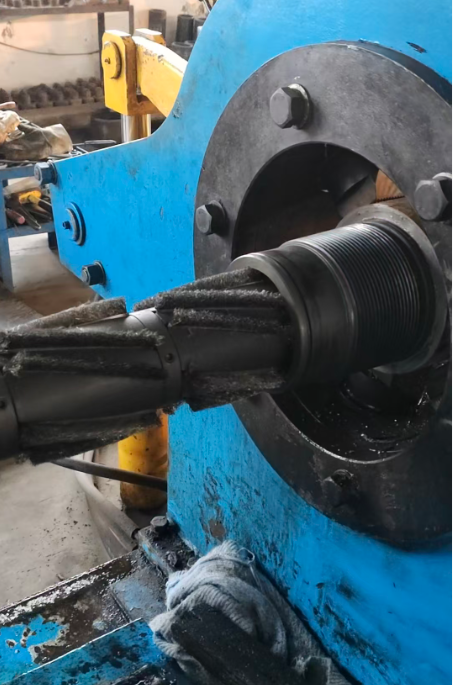
\includegraphics[height=8.0cm]{figure/chapter3/part1-3in1/brush-pipe-test-1.png}}
	\hfill
	\subfloat[毛刷短节在管内往复活动]{%
	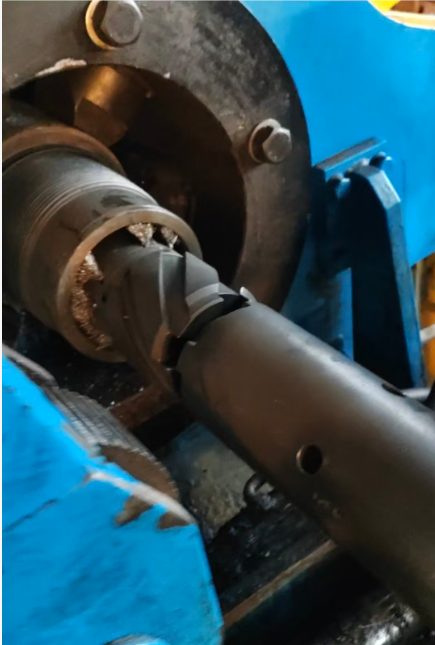
\includegraphics[height=8.0cm]{figure/chapter3/part1-3in1/brush-pipe-test-2.png}}
	\caption{毛刷刮管器通过性试验}
	\label{fig:3in1_brush_test}
\end{figure}

由图\ref{fig:3in1_brush_test}可见，毛刷短节装配后能够顺利进入试验管段，并在管内往复活动过程中与管壁保持接触。所测摩擦力可作为判断毛刷压缩量是否合适、工具在套管内是否易于遇阻的依据。

\subsubsection{脉冲器试验}

脉冲器试验采用打压泵打压。打压3\,min内，泵压波动范围为$0\sim4$\,MPa；当排量达到300\,L/min时，脉冲器开始振动，实测振动频率为$15\sim20$\,Hz，工作状态如图\ref{fig:3in1_pulser_test}所示。

\begin{figure}[htbp]
	\centering
	\subfloat[脉冲器试验台架安装]{%
	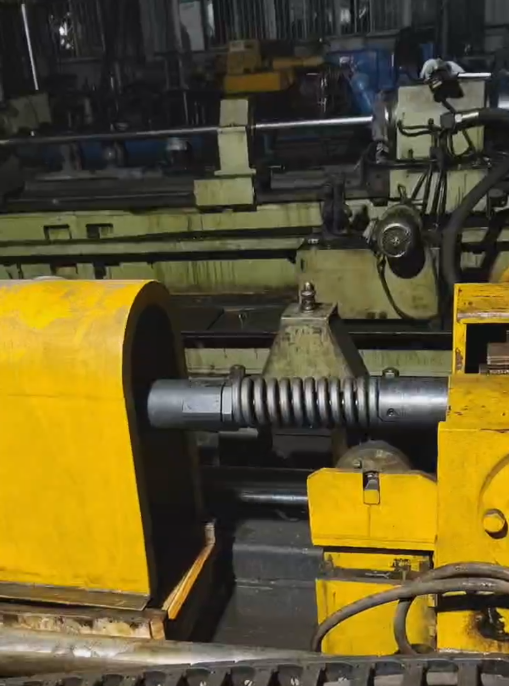
\includegraphics[height=8.0cm]{figure/chapter3/part1-3in1/pulser-test-bench-1.png}}
	\hfill
	\subfloat[脉冲器出水振动状态]{%
	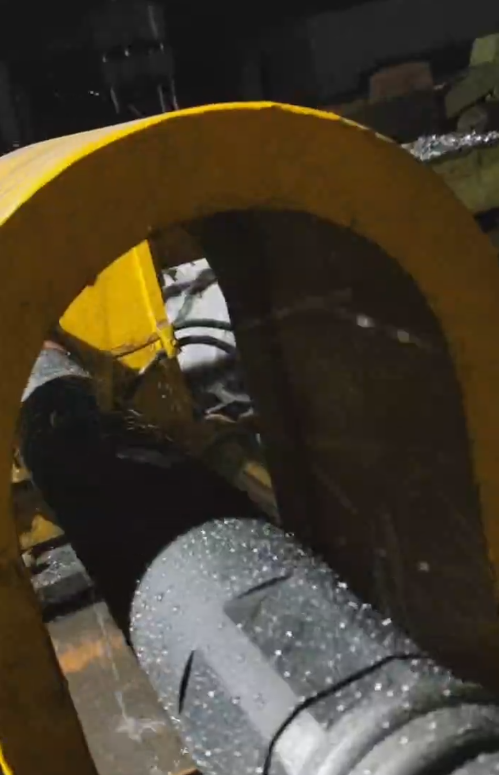
\includegraphics[height=8.0cm]{figure/chapter3/part1-3in1/pulser-jetting-test.png}}
	\caption{脉冲器试验状态}
	\label{fig:3in1_pulser_test}
\end{figure}

脉冲器出厂前单独试验的测试数据见表\ref{tab:3in1_pulser_factory}。

\begin{table}[htbp]
    \centering
    \caption{脉冲器出厂试验数据}
    \label{tab:3in1_pulser_factory}
    \small % 列数较多，适当缩小字号，避免超出正文版心
    \setlength{\tabcolsep}{3pt}
    \renewcommand{\arraystretch}{1.4}
    \begin{tabular*}{\textwidth}{@{\extracolsep{\fill}}ccccccc@{}}
        \toprule % 顶线
        型号 & 名称 & \begin{tabular}[c]{@{}c@{}}喷嘴直径\\ ($\times$2, mm)\end{tabular} & 
        \begin{tabular}[c]{@{}c@{}}压力\\ (MPa)\end{tabular} & 
        \begin{tabular}[c]{@{}c@{}}流量\\ (L/min)\end{tabular} & 状态 & 备注 \\
        \midrule % 栏目线
        \multirow{3}{*}{MCQ105} & \multirow{3}{*}{4\,1/8\,英寸脉冲短节} & 3.175 & 2 & 200 & 未震动 & 脉冲1 \\
        & & 3.175 & 6 & 420 & 开始震动 & 脉冲2 \\
        & & 3.175 & 8 & 480 & \begin{tabular}[c]{@{}c@{}}弹簧压并不回弹\\ （泄压后回弹）\end{tabular} & 脉冲3 \\
        \bottomrule % 底线
    \end{tabular*}
\end{table}

由表\ref{tab:3in1_pulser_factory}可见，出厂试验时泵压在$6\sim8$\,MPa范围内脉冲器可保持低频往复运动；当泵压大于8\,MPa时，弹簧被压并而无法回弹。分析认为，其原因可能为喷嘴直径偏小，活塞滑过喷嘴孔后喷嘴泄流泄压不明显，弹簧所受作用力减小幅度不足，因而无法复位。

针对上述问题，脉冲器的优化方案为：更换大口径喷嘴，并加大弹簧预压力，保证泄压过程明显、回弹弹力充足。

此外，本次测试中脉冲器在300\,L/min时即已起振，低于出厂单独试验的起振排量（420\,L/min），两者试验条件（管串组合与背压）不同，其对应关系尚需在整机试验中进一步标定。

\subsubsection{液压刮管器试验}

测试前先在井口投球，钢球直径为$\phi$28\,mm。使用泵车打压，泵压升至15\,MPa时刮刀无动作，停泵泄压；随后将泵压升至17\,MPa，刮刀张开，张开行程约8\,mm。停泵后泵压下降至0\,MPa，刮刀未能自行回收，拆下管线后刮刀才回收，刮刀状态如图\ref{fig:3in1_scraper_test}所示。

\begin{figure}[htbp]
	\centering
	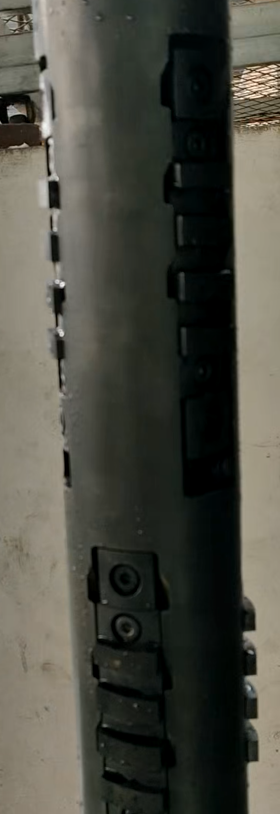
\includegraphics[width=3.4cm]{figure/chapter3/part1-3in1/hydraulic-scraper-blades.png}
	\caption{液压刮管器刮刀状态}
	\label{fig:3in1_scraper_test}
\end{figure}

液压刮管器出厂前静液压试验的测试数据见表\ref{tab:3in1_scraper_factory}。

\begin{table}[htbp]
    \centering
    \caption{液压刮管器出厂试验数据}
    \label{tab:3in1_scraper_factory}
    \small % 列数较多，适当缩小字号，避免超出正文版心
    \setlength{\tabcolsep}{3pt}
    \renewcommand{\arraystretch}{1.4}
    \begin{tabular*}{\textwidth}{@{\extracolsep{\fill}}ccccccc@{}}
        \toprule % 顶线
        型号 & 名称 & \begin{tabular}[c]{@{}c@{}}激活钢球\\ (mm)\end{tabular} & 
        \begin{tabular}[c]{@{}c@{}}激活压力\\ (MPa)\end{tabular} & 
        \begin{tabular}[c]{@{}c@{}}剪切螺钉\\ 数量\end{tabular} & 
        \begin{tabular}[c]{@{}c@{}}张开外径\\ (mm)\end{tabular} & 备注 \\
        \midrule % 栏目线
        YYGG105 & 4\,英寸液压刮管器 & $\phi$28 & 40 & 12（钢） & 130 & 刮壁器1 \\
        \multicolumn{2}{c}{出厂设置} & --- & 20 & 8（铜） & --- & 刮壁器2 \\
        \bottomrule % 底线
    \end{tabular*}
\end{table}

第一次静液压试验采用钢制剪钉，投球后泵压达到40\,MPa时剪钉剪断、刮刀张开；此后改用铜制剪钉，剪切压力为20\,MPa$\pm$2\,MPa。第二个$\phi$32\,mm钢球仅在需要强制回收刮刀时投放，投放后水眼封闭，因此可将上球座改为滑套结构，使投球后水眼保持畅通。

东营试验基地试验中，投球后泵压升至17\,MPa时销钉即已剪断，但刮刀未完全伸出；刮刀完全张开所需泵压≥2\,MPa，此时泵压是否达到要求尚不确定。停泵后刮刀未收回，可能为刮刀滑槽内有异物或机械卡滞所致；卸掉水龙带时工具产生轻微振动，滑槽恢复顺畅后刮刀才顺利回位。

\subsubsection{旋转喷头试验}

试验使用泵车供液。先将排量调至0.15\,m$^3$/min，以较低排量循环，旋转喷头出水但未旋转；随后逐步提高排量，最高升至0.45\,m$^3$/min，旋转喷头仍只出水而不旋转，停泵，测试结束。旋转喷头试验状态如图\ref{fig:3in1_nozzle_test}所示。

\begin{figure}[htbp]
	\centering
	\subfloat[试验前喷头与工具串连接]{%
	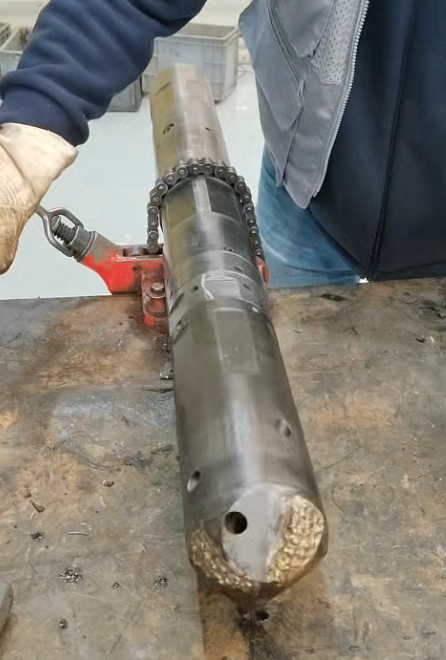
\includegraphics[height=8.0cm]{figure/chapter3/part1-3in1/rotary-nozzle-makeup.png}}
	\hfill
	\subfloat[试验中喷头射流状态]{%
	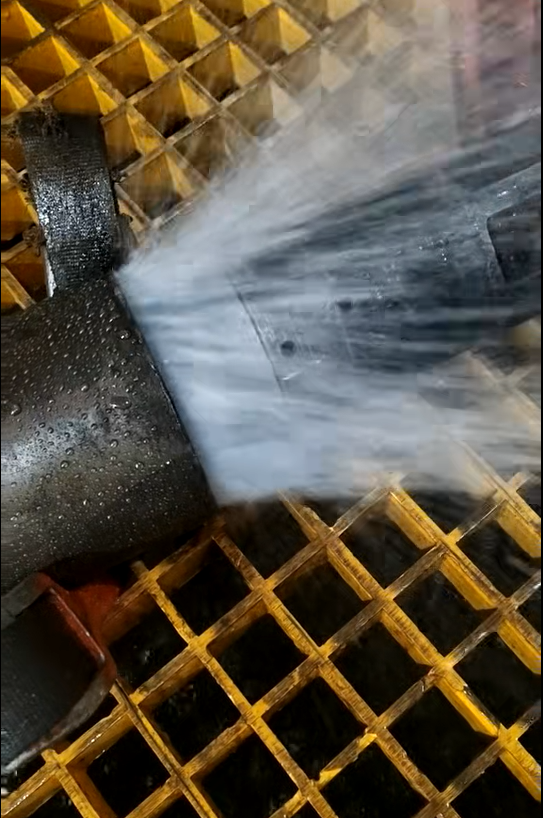
\includegraphics[height=8.0cm]{figure/chapter3/part1-3in1/rotary-nozzle-jetting.png}}
	\caption{旋转喷头试验状态}
	\label{fig:3in1_nozzle_test}
\end{figure}

旋转喷头出厂试验数据见表\ref{tab:3in1_nozzle_factory}。

\begin{table}[htbp]
    \centering
    \caption{旋转喷头出厂试验数据}
    \label{tab:3in1_nozzle_factory}
    \small % 列数较多，适当缩小字号，避免超出正文版心
    \setlength{\tabcolsep}{3pt}
    \renewcommand{\arraystretch}{1.4}
    \begin{tabular*}{\textwidth}{@{\extracolsep{\fill}}cccccccc@{}}
        \toprule % 顶线
        型号 & 名称 & \begin{tabular}[c]{@{}c@{}}喷嘴直径\\ (mm)\end{tabular} & 
        \begin{tabular}[c]{@{}c@{}}喷嘴\\ 数量\end{tabular} & 
        \begin{tabular}[c]{@{}c@{}}工作压力\\ (MPa)\end{tabular} & 
        \begin{tabular}[c]{@{}c@{}}工作流量\\ (L/min)\end{tabular} & 
        \begin{tabular}[c]{@{}c@{}}转速\\ (r/min)\end{tabular} & 备注 \\
        \midrule % 栏目线
        XZPT105 & 4\,1/8\,英寸旋转喷头 & 3.175 & 7 & $\ge2$ & $\ge350$ & $10\sim300$ & 旋转喷头1 \\
        \multicolumn{2}{c}{二次试验工具串} & 3.175 & 5（2个未装） & $\ge3$ & $\ge450$ & $10\sim300$ & 旋转喷头3 \\
        \bottomrule % 底线
    \end{tabular*}
\end{table}

旋转喷头单独试验时，排量达到$350\sim400$\,L/min即开始旋转，此时泵压约为2.2\,MPa；接入刮刀与脉冲器后，管内压降发生变化，拆掉2个喷射喷嘴并提高排量、使泵压不低于3\,MPa后，喷头才开始转动。本次东营基地试验中喷头未能转动，可能与上部工具压耗过大有关。试验过程中应保证泵压不低于3\,MPa，或将旋转喷头头部下入套管内，以增大喷射孔的反冲力矩。

\subsubsection{试验结论与改进措施}

综合各模块的试验结果，可得如下结论：

\begin{itemize}
	\item 毛刷刮管器装配后可通过$\phi$114\,mm试验管段并往复活动，毛刷与管壁保持接触，满足入井刮刷对通过性的要求；
	\item 脉冲器在300\,L/min、泵压波动$0\sim4$\,MPa条件下可正常起振，振动频率为$15\sim20$\,Hz；但当泵压大于8\,MPa时弹簧压并不回弹，需通过更换大口径喷嘴、加大弹簧预压力予以改进；
	\item 液压刮管器在15\,MPa时未动作、17\,MPa时刮刀张开，张开行程约8\,mm；停泵后刮刀不能自行回收，需拆卸管线后才能回位，反映剪钉剪切压力与刮刀回位机构仍需优化；
	\item 旋转喷头单独试验时，在$350\sim400$\,L/min、2.2\,MPa条件下即可旋转；接入刮刀与脉冲器后需在泵压不低于3\,MPa时才转动；东营基地试验中因上部压耗过大未能转动，需在整机联调中重新匹配排量与压耗。
\end{itemize}

针对试验中暴露的问题，后续将从喷嘴通径、弹簧预压力、剪钉配置与球座结构以及喷头压耗匹配等方面对工具进行改进，并在整机联调中复测验证。
